% Options for packages loaded elsewhere
\PassOptionsToPackage{unicode}{hyperref}
\PassOptionsToPackage{hyphens}{url}
%
\documentclass[
]{article}
\usepackage{amsmath,amssymb}
\usepackage{lmodern}
\usepackage{iftex}
\ifPDFTeX
  \usepackage[T1]{fontenc}
  \usepackage[utf8]{inputenc}
  \usepackage{textcomp} % provide euro and other symbols
\else % if luatex or xetex
  \usepackage{unicode-math}
  \defaultfontfeatures{Scale=MatchLowercase}
  \defaultfontfeatures[\rmfamily]{Ligatures=TeX,Scale=1}
\fi
% Use upquote if available, for straight quotes in verbatim environments
\IfFileExists{upquote.sty}{\usepackage{upquote}}{}
\IfFileExists{microtype.sty}{% use microtype if available
  \usepackage[]{microtype}
  \UseMicrotypeSet[protrusion]{basicmath} % disable protrusion for tt fonts
}{}
\makeatletter
\@ifundefined{KOMAClassName}{% if non-KOMA class
  \IfFileExists{parskip.sty}{%
    \usepackage{parskip}
  }{% else
    \setlength{\parindent}{0pt}
    \setlength{\parskip}{6pt plus 2pt minus 1pt}}
}{% if KOMA class
  \KOMAoptions{parskip=half}}
\makeatother
\usepackage{xcolor}
\usepackage[margin=1in]{geometry}
\usepackage{graphicx}
\makeatletter
\def\maxwidth{\ifdim\Gin@nat@width>\linewidth\linewidth\else\Gin@nat@width\fi}
\def\maxheight{\ifdim\Gin@nat@height>\textheight\textheight\else\Gin@nat@height\fi}
\makeatother
% Scale images if necessary, so that they will not overflow the page
% margins by default, and it is still possible to overwrite the defaults
% using explicit options in \includegraphics[width, height, ...]{}
\setkeys{Gin}{width=\maxwidth,height=\maxheight,keepaspectratio}
% Set default figure placement to htbp
\makeatletter
\def\fps@figure{htbp}
\makeatother
\setlength{\emergencystretch}{3em} % prevent overfull lines
\providecommand{\tightlist}{%
  \setlength{\itemsep}{0pt}\setlength{\parskip}{0pt}}
\setcounter{secnumdepth}{-\maxdimen} % remove section numbering
\usepackage{expl3}
\usepackage{xparse}
\usepackage{tcolorbox}
\usepackage{amsmath,amsfonts,amsthm}
\usepackage{wrapfig}
\definecolor{gssmidblue}{RGB}{32, 115, 188}
\usepackage{booktabs}
\usepackage{longtable}
\usepackage{array}
\usepackage{multirow}
\usepackage{wrapfig}
\usepackage{float}
\usepackage{colortbl}
\usepackage{pdflscape}
\usepackage{tabu}
\usepackage{threeparttable}
\usepackage{threeparttablex}
\usepackage[normalem]{ulem}
\usepackage{makecell}
\usepackage{xcolor}
\ifLuaTeX
  \usepackage{selnolig}  % disable illegal ligatures
\fi
\IfFileExists{bookmark.sty}{\usepackage{bookmark}}{\usepackage{hyperref}}
\IfFileExists{xurl.sty}{\usepackage{xurl}}{} % add URL line breaks if available
\urlstyle{same} % disable monospaced font for URLs
\hypersetup{
  pdftitle={School Places Scorecard},
  hidelinks,
  pdfcreator={LaTeX via pandoc}}

\title{School Places Scorecard}
\author{}
\date{\vspace{-2.5em}}

\begin{document}
\maketitle

\hypertarget{data-for-primary-schools-in-durham}{%
\section{Data for Primary Schools in
Durham}\label{data-for-primary-schools-in-durham}}

\makebox[1.00\linewidth]{
\centering


\begin{tcolorbox}[colback=gssmidblue, 
 leftright skip=0.1cm,
 coltext=white, 
 halign=left, 
 fontupper={\Huge \bfseries},
 fontlower={\large \bfseries},
 sharp corners, 
 colframe=gssmidblue,
 width=0.49\linewidth,
 boxrule=0pt 
 ]
£21million
\tcblower
Total primary and secondary basic need funding 2011-22
\end{tcolorbox}


\begin{tcolorbox}[colback=gssmidblue, 
 leftright skip=0.1cm,
 coltext=white, 
 halign=left, 
 fontupper={\Huge \bfseries},
 fontlower={\large \bfseries},
 sharp corners, 
 colframe=gssmidblue,
 width=0.49\linewidth,
 boxrule=0pt 
 ]
10\%
\tcblower
Growth in primary, pupil numbers 2009/10 to 2021-22
\end{tcolorbox}
}

\hypertarget{quantity}{%
\subsection{Quantity}\label{quantity}}

\hypertarget{places-created-since-2009-10-places-planned-to-2021-22-and-estimated-place-pressure-in-2021-22}{%
\subsubsection{Places created since 2009-10, places planned to 2021-22
and estimated place pressure in
2021-22}\label{places-created-since-2009-10-places-planned-to-2021-22-and-estimated-place-pressure-in-2021-22}}

A local authority can have both `spare places' and `additional places
needed' due to localised or specific year group demand

\makebox[1.0\linewidth]{
\centering
\begin{tcolorbox}[colback=gssmidblue, 
 leftright skip=0.1cm,
 coltext=white, 
 halign=left, 
 fontupper={\Huge \bfseries},
 fontlower={\large \bfseries},
 sharp corners, 
 colframe=gssmidblue,
 width=0.49\linewidth,
 boxrule=0pt 
 ]
180
\tcblower
Estimated additional primary places to meet demand in 2021-22 
\end{tcolorbox}
\begin{tcolorbox}[colback=gssmidblue, 
 leftright skip=0.1cm,
 coltext=white, 
 halign=left, 
 fontupper={\Huge \bfseries},
 fontlower={\large \bfseries},
 sharp corners, 
 colframe=gssmidblue,
 width=0.49\linewidth,
 boxrule=0pt 
 ]
15\%
\tcblower
Estimated percentage of spare primary places in 2021-22
\end{tcolorbox}
}

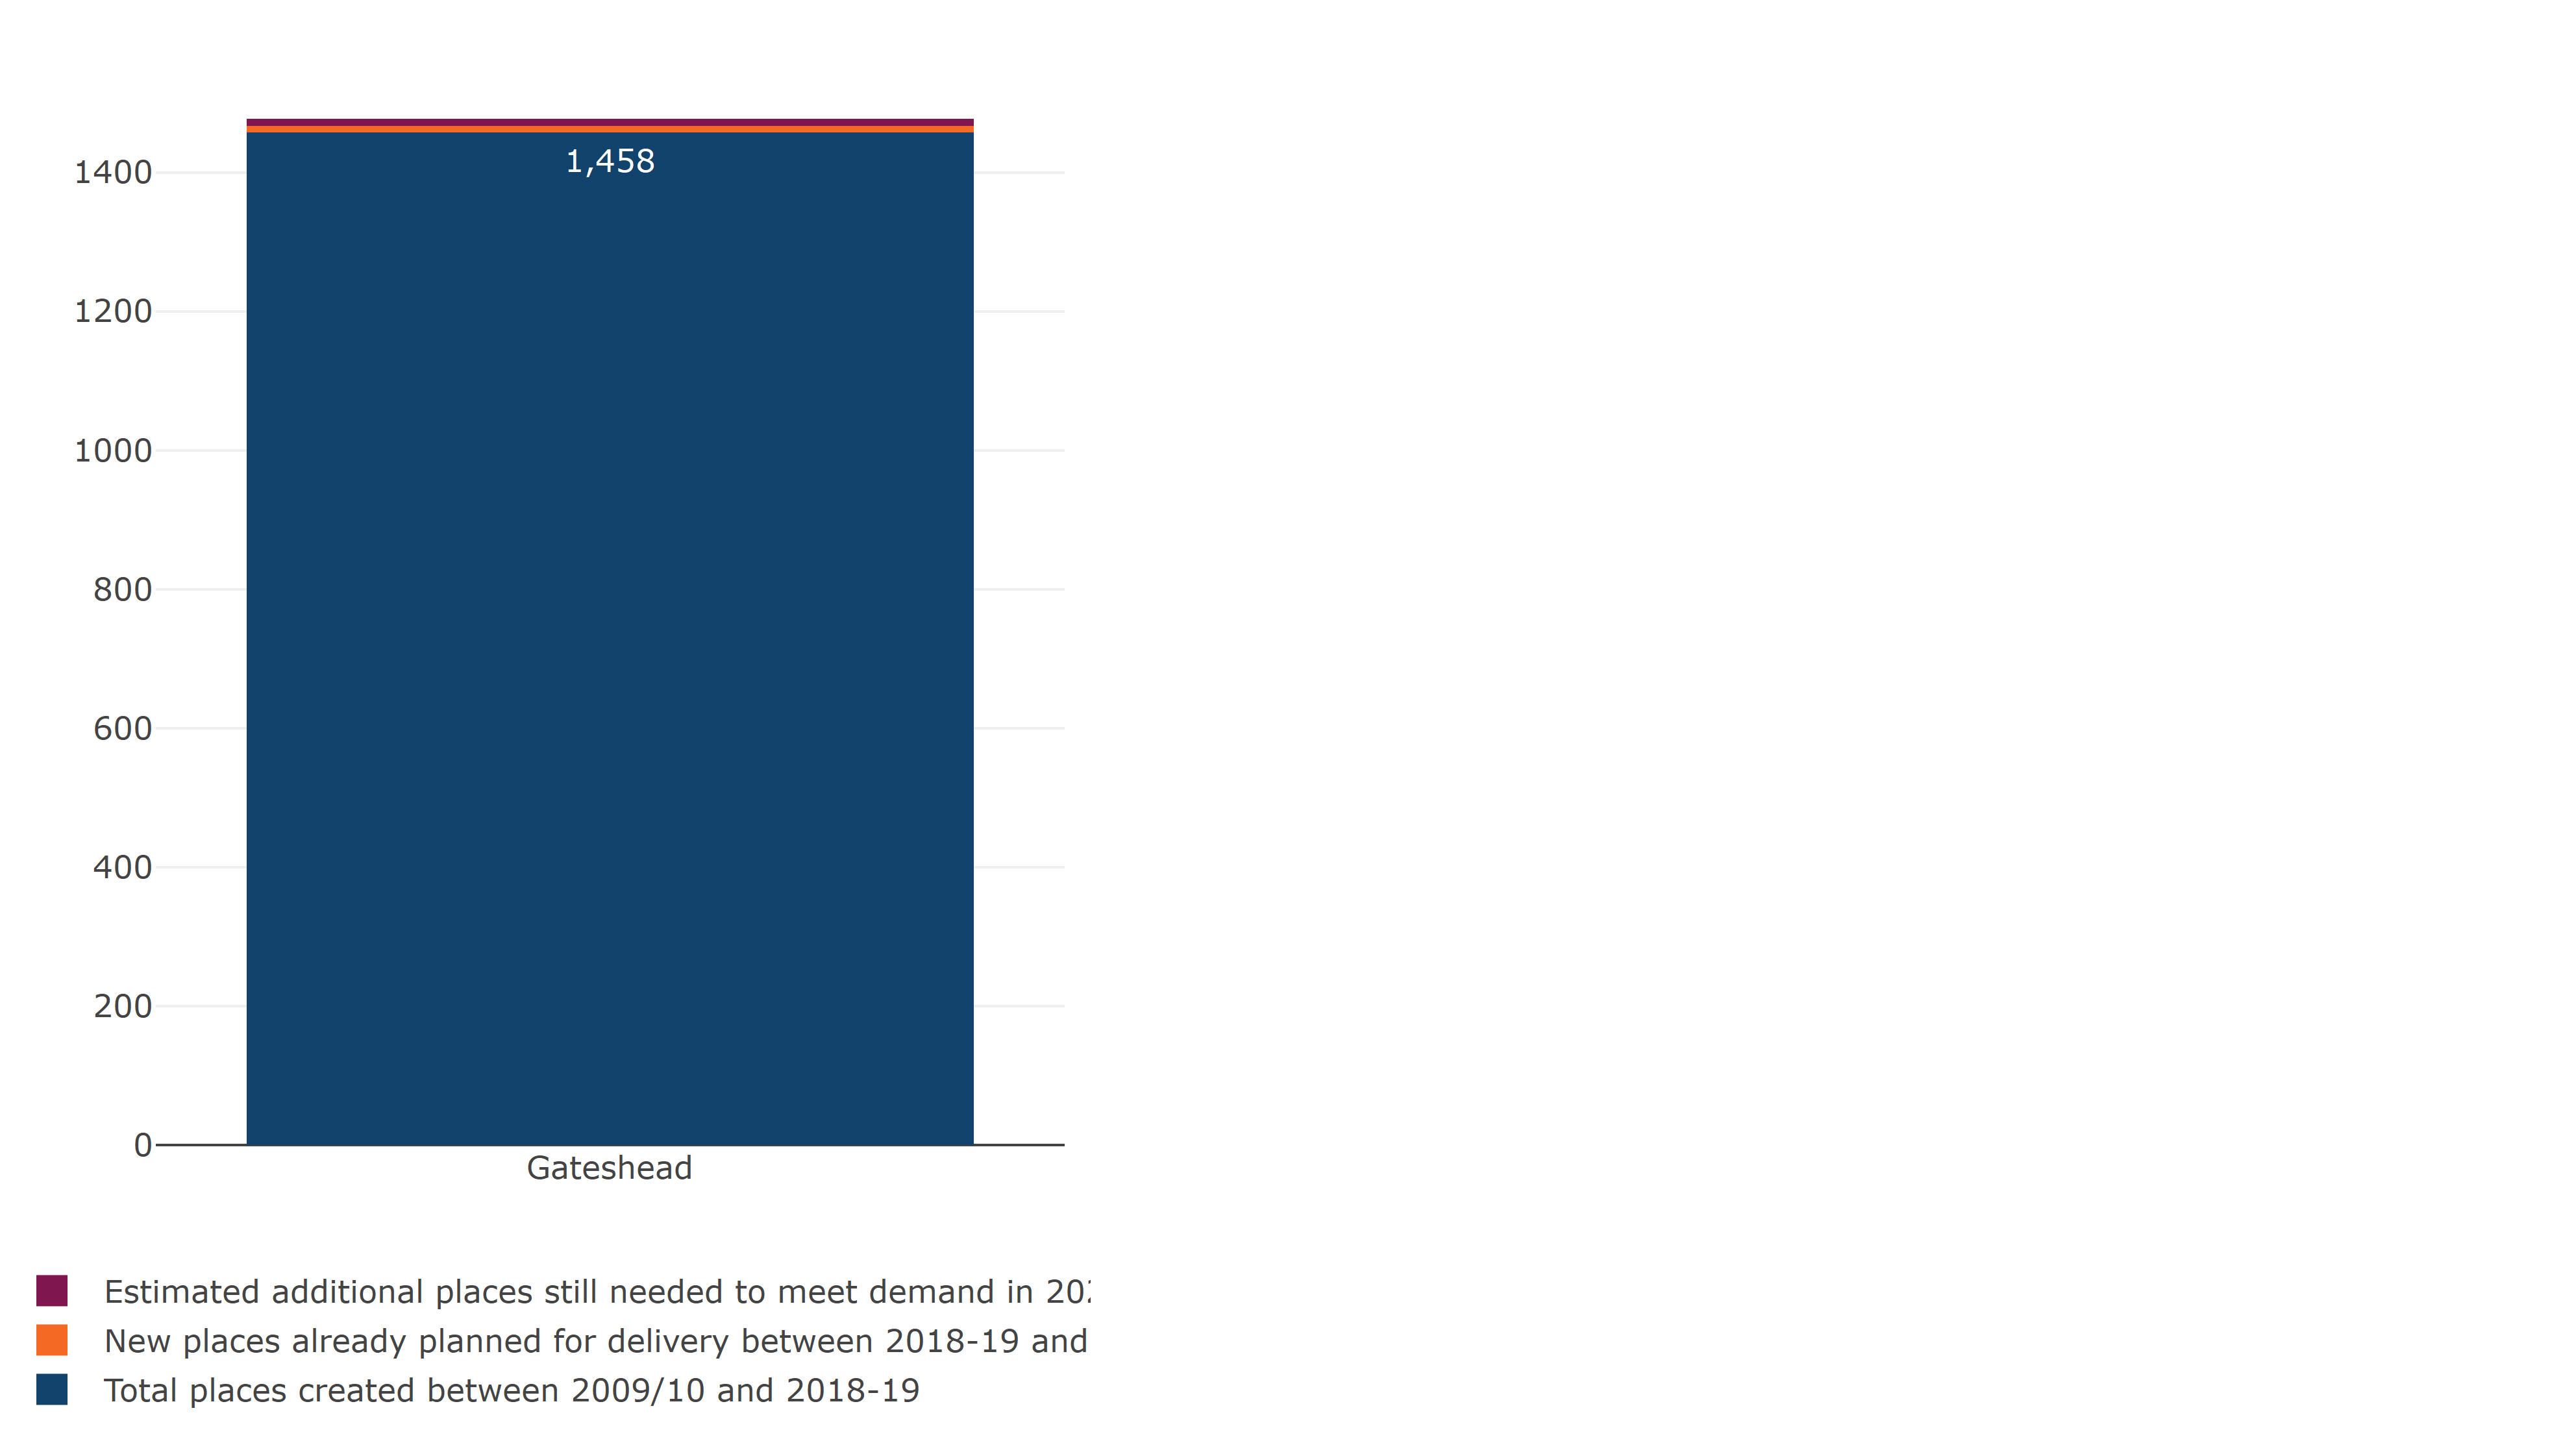
\includegraphics[width=1\linewidth,height=1\textheight]{Summary_scorecard_files/figure-latex/quantity_b-1}

\hypertarget{preference}{%
\subsection{Preference}\label{preference}}

\hypertarget{proportion-of-applicants-who-received-an-offer-of-one-of-their-top-three-preference-schools-for-september-2019-entry}{%
\subsubsection{Proportion of applicants who received an offer of one of
their top three preference schools for September 2019
entry}\label{proportion-of-applicants-who-received-an-offer-of-one-of-their-top-three-preference-schools-for-september-2019-entry}}

\makebox[1.0\linewidth]{
\centering
\begin{tcolorbox}[colback=gssmidblue, 
 leftright skip=0.1cm,
 coltext=white, 
 halign=left, 
 fontupper={\Huge \bfseries},
 fontlower={\large \bfseries},
 sharp corners, 
 colframe=gssmidblue,
 width=0.49\linewidth,
 boxrule=0pt 
 ]
97.5\%
\tcblower
Percentage of applicants who recieved an offer of one of their top three preferred primary schools in England
\end{tcolorbox}
\begin{tcolorbox}[colback=gssmidblue, 
 leftright skip=0.1cm,
 coltext=white, 
 halign=left, 
 fontupper={\Huge \bfseries},
 fontlower={\large \bfseries},
 sharp corners, 
 colframe=gssmidblue,
 width=0.49\linewidth,
 boxrule=0pt 
 ]
 99.3 \%
\tcblower
Percentage of applicants who recieved an offer of one of their top three preferred  primary  places in  2021-22  in  Durham 
\end{tcolorbox}
}

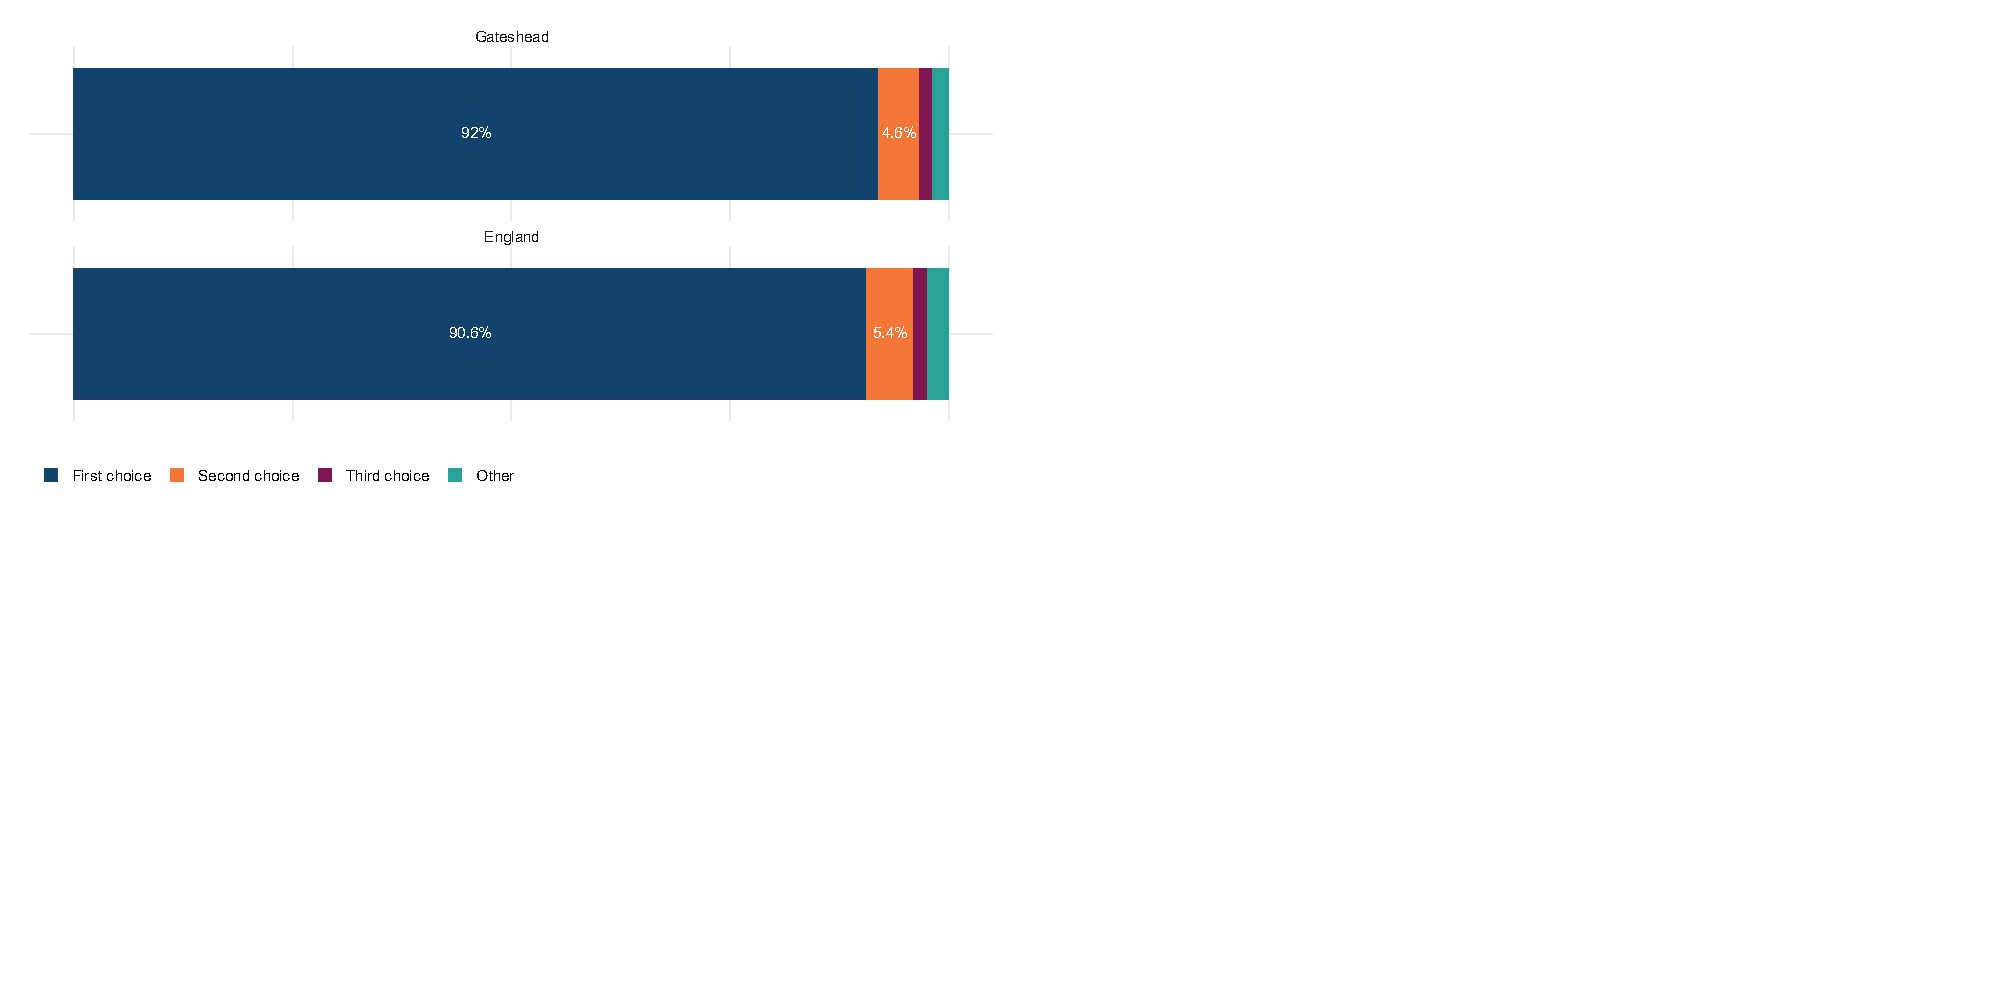
\includegraphics[width=1.3\linewidth]{Summary_scorecard_files/figure-latex/preference_barchart-1}

\hypertarget{quality}{%
\subsection{Quality}\label{quality}}

\hypertarget{quality-of-places-created-between-2017-18-and-2018-19-based-on-ofsted}{%
\subsubsection{Quality of places created between 2017-18 and 2018-19,
based on
Ofsted:}\label{quality-of-places-created-between-2017-18-and-2018-19-based-on-ofsted}}

\begin{verbatim}
## [1] "Percentage of new places created in good and outstanding primary schools in Durham: 100%"
\end{verbatim}

\begin{verbatim}
## [1] "Percentage of new places in good and outstanding primary schools in England: 91%"
\end{verbatim}

\begin{verbatim}
## [1] "LA Rank out of 120 LAs that created new places between 2017-18 and 2018-19 (ranks can be tied):"
\end{verbatim}

\begin{verbatim}
## [1] "1"
\end{verbatim}

\textbackslash makebox{[}1.0\linewidth{]}\{ \centering

\begin{tcolorbox}[colback=gssmidblue, 
 leftright skip=0.1cm,
 coltext=white, 
 halign=left, 
 fontupper={\Huge \bfseries},
 fontlower={\large \bfseries},
 sharp corners, 
 colframe=gssmidblue,
 width=0.32\linewidth,
 boxrule=0pt 
 ]
97.5\%
\tcblower
Percentage of applicants who recieved an offer of one of their top three preferred primary schools in England
\end{tcolorbox}
\begin{tcolorbox}[colback=gssmidblue, 
 leftright skip=0.1cm,
 coltext=white, 
 halign=left, 
 fontupper={\Huge \bfseries},
 fontlower={\large \bfseries},
 sharp corners, 
 colframe=gssmidblue,
 width=0.32\linewidth,
 boxrule=0pt 
 ]
 99.3 \%
\tcblower
Percentage of applicants who recieved an offer of one of their top three preferred  primary  places in  2021-22  in  Durham 
\end{tcolorbox}\begin{tcolorbox}[colback=gssmidblue, 
 leftright skip=0.1cm,
 coltext=white, 
 halign=left, 
 fontupper={\Huge \bfseries},
 fontlower={\large \bfseries},
 sharp corners, 
 colframe=gssmidblue,
 width=0.32\linewidth,
 boxrule=0pt 
 ]
 99.3 \%
\tcblower
Percentage of applicants who recieved an offer of one of their top three preferred  primary  places in  2021-22  in  Durham 
\end{tcolorbox}

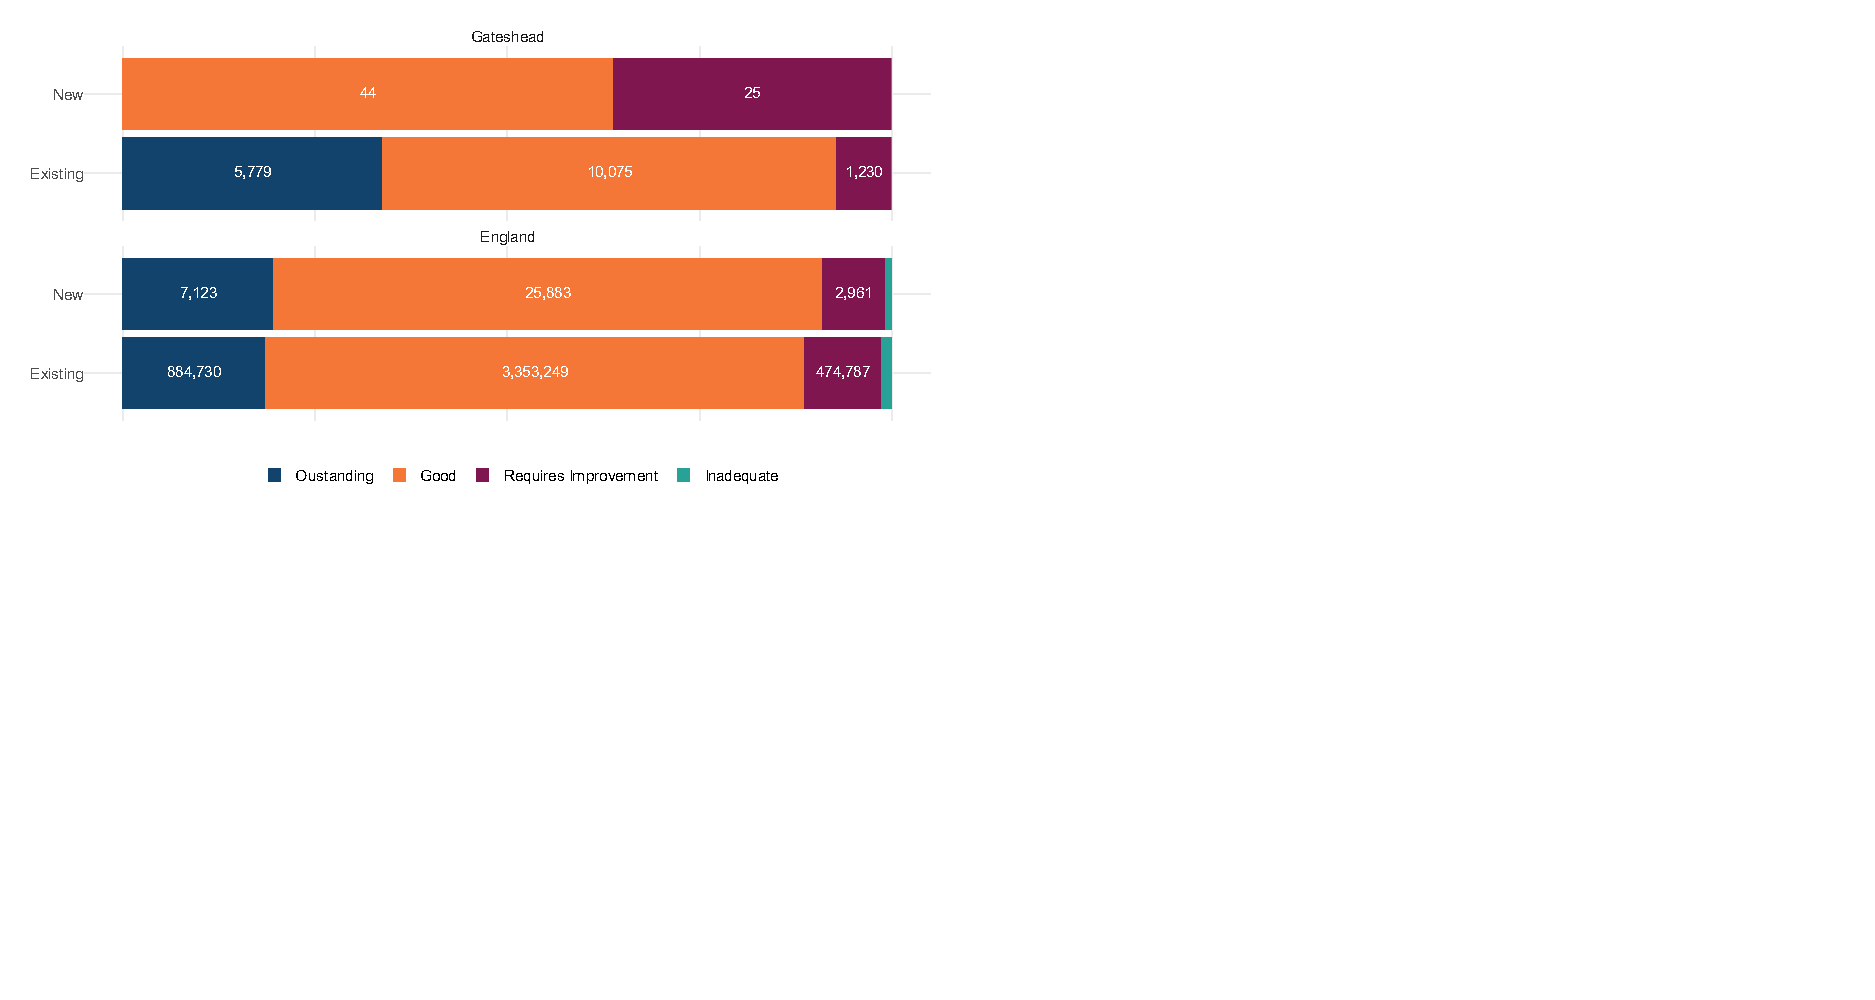
\includegraphics{Summary_scorecard_files/figure-latex/quality_chart-1.pdf}

New places with no rating = NA

\hypertarget{cost}{%
\subsection{Cost}\label{cost}}

\end{document}
